\documentclass[a4paper,11pt, twocolumn]{article}
%\usepackage[T1]{fontenc} %for å bruke æøå
\usepackage[utf8]{inputenc}
\usepackage[T1]{fontenc}
\usepackage[norsk]{babel}
\usepackage{graphicx} %for å inkludere grafikk
\usepackage{verbatim} %for å inkludere filer med tegn LaTeX ikke liker
\usepackage{mathpazo}
\usepackage{mathtools}
\usepackage{csquotes}
\usepackage{tikz}
\usepackage{listings}
\usepackage{booktabs}
\usepackage{todonotes}
\usepackage[backend=biber]{biblatex}
\usepackage{caption} 
\usepackage{parboxx}
\hyphenpenalty=750
\captionsetup[table]{skip=10pt}

%\addbibresource{solceller.bib}

\lstset{language=Matlab, commentstyle=\textcolor[rgb]{0.00,0.50,0.00}, keepspaces=true, columns=flexible, basicstyle=\footnotesize, keywordstyle=\color{blue}, showstringspaces=false, inputencoding=ansinew}

\title{Rapport 3 FYS2150\\Solcellen}

\author{Eivind Brox}
\date{\today}

\begin{document}

\maketitle
\listoftodos
\begin{abstract}

\end{abstract}

\section{Introduksjon}
Energi er et viktig tema innenfor vitenskap, økonomi og politikk. Det diskuteres stadig hvilke kilder det skal satses på, og hvilke som bør fases ut til fordel for et mer menneskevennlig klima på jorden. 

I utgangspunktet er det bare tre kilder til energi som påvirker jorden. Solen er den som bidrar sterkest til energien mennesker nyttiggjør seg av idag. Geotermisk energi fra jorden indre prosesser utnyttes i mindre grad, og energi fra kosmisk stråling har lite potensial.

Solen varmer opp og skaper bevegelse i havene, den setter lufta i bevegelse og får planter til å vokse. Alle disse effektene kan brukes til å indirekte høste energi fra solen. Det kunne kanskje være interessant å høste energien mer direkte fra solen og kvitte seg med flere av mellomleddene?

Solceller lar oss gjøre nettopp dette. Mellomledd er fortsatt til stede, men energien er momentant tilgjengelig så lenge solen skinner. Utfordringer knyttet til solcelleteknologi dreier seg om å effektivisere produksjon og drift. I denne rapporten ser vi nettopp på solcellens virkemåte i forhold til hvordan cellene kobles sammen, hvilken last som bør brukes for å oppnå maksimal effekt og hvilke bølgelengder som gir størst effektivitet.   
\section{Teori}
Ideelle motstander virker under Ohms lov, spenning er lik strøm multiplisert med motstand, $V=RI$. Denne forenklingen benytter vi i dette arbeidet. I tillegg benytter vi at effekt er spenning multiplisert med strøm, $P = VI$.

For arbeidet med å finne maksimal effekt vi kan få ut fra to solceller under forskjellige koblinger og lysforhold benytter vi en forenkling for å slippe å finne strøm-spenning karakteristikken for alle forholdene.

\begin{figure}[!ht]
	\includegraphics[width = 0.5\textwidth]{stromSpenningSolcelle.png}
	\caption{Strøm-spenning-karakteristikk for en solcelle. Det skraverte rektangelet tilsvarer effekten solcellen leverer.}
	\label{fig:powerCurrentVoltage}
\end{figure}

I figur \ref{fig:powerCurrentVoltage} kan vi regne ut effekten som arealet av det skraverte rektangelet. Vi benytter at forholdet mellom dette arealet på sitt største og arealet til rektangelet som omslutter hele karakteristikken er tilnærmet konstant. Vi har dermed 
\begin{equation}
	\frac{P_\text{max}}{V_\text{oc}I_\text{sc}}\approx\text{konstant}
\end{equation}
der $P_\text{max}$ er den maksimale effekten ved optimal lastmotstand, $V_\text{oc}$ er spenningen over lasten ved åpen krets, og $I_\text{sc}$ er strømmen gjennom solcellen når kretsen kortsluttes.

Forholdet mellom de optimale effektene for to oppsett blir dermed
\begin{equation}
	\frac{(P_\text{max})_1}{(P_\text{max})_2} \approx \frac{(V_\text{oc}I_\text{sc})_1}{(V_\text{oc}I_\text{sc})_2}
	\label{eq:forhold}
\end{equation}
\todo[inline]{Kanskje noe om hvordan solcellen fungerer!}
\section{Eksperimentelt}
Mye av utstyret brukt til de forskjellige forsøkene var likt. Det generelle utstyret er derfor listet opp her.

{\bf Utstyr}
\begin{itemize}
	\item 2 solceller
	\item 2 Fluke 45 multimetere
	\item Dekademotstand
	\item Lysbildeframviser (lyskilde)
	\item Optisk benk
\end{itemize}

Det generelle oppsettet var som i figur \ref{fig:oppsett}, hvor solarimeteret kunne byttes ut med en annen solcelle. Det første vi gjorde var å stille inn avstanden mellom solcellen og lyskilden slik at lyset fra lyskilden akkurat ville dekke to solceller som stod ved siden av hverandre. Denne avstanden brukte vi for resten av eksperimentene.
\begin{figure}[ht!]
	\includegraphics[width = 0.5\textwidth]{optiskBenk.png}
	\caption{Generelt oppsett for forsøkene}
	\label{fig:oppsett}
\end{figure}
Strømmene gjennom solcellene finner vi ved Ohms lov og måling av spenning over dekademotstanden, slik at $I = V_L/R_L$. Dekademotstanden fungerer som lastmotstand, $R_L$, for solcellen, og $V_L$ er spenningen over denne lasten (se for eksempel figur \ref{fig:solcelleMedSpenning}). Dette gjorde vi i stedet for å måle strømmen direkte med et multimeter fordi solcellen ofte krever lavere lastmotstand enn den indre motstanden i multimeteret.
\subsection{Solcellen som halvlederdiode}
Vi finner strøm-spenning-karakteristikken til solcellen vår under belysning, med og uten påtrykt spenning over cellen. Dette gjør vi ved å måle strøm gjennom og spenning over solcellen ved forskjellige lastmotstandsverdier. 
\subsubsection{Med påtrykt spenning}
Den første strøm-spenning-karakteristikken finner vi med påtrykt spenning over solcellen. Den påtrykte spenningen lot vi være 5V for alle målingene. Vi brukte fastspenningsuttakene ettersom disse har mulighet til å levere høyere strøm enn de variable. Vi koblet utstyr som i figur \ref{fig:solcelleMedSpenning} først, og utførte endel målinger for dette oppsettet. Etter dette snudde vi polariteten til den påtrykte spenningen. Vi målte altså først for strøm i solcellens lederetning, før vi gjorde målinger for strøm i sperreretning. Vi forsøkte å velge smarte verdier for lastmotstanden for å dekke de områdene med størst endring med flest målinger.

\begin{figure}[!ht]
	\includegraphics[width = 0.5\textwidth]{solcelleMedSpenning.png}
	\caption{Koblingsskjema for målinger av strøm-spenning-karakteristikken til en solcelle med påtrykt spenning.}
	\label{fig:solcelleMedSpenning}
\end{figure}

\subsubsection{Uten påtrykt spenning}
Videre fjernet vi spenningen som var påtrykt solcellen (koblet ut spenningskilden, $\varepsilon$ i figur \ref{fig:solcelleMedSpenning}, og koblet sammen ledningene). Omtrent samme framgangsmåte som i forrige seksjon ble benyttet.
\subsection{Solcellens optimale belastning}
Det er interessant å se på hva slags forhold en solcelle arbeider best under.
For å undersøke solcellens optimale belastning sammenlignes data fra målingene gjort med full belysning uten påtrykt spenning med nye data med redusert belysning. Måten vi reduserte belysningen på var ved å rotere solcellen slik at spenningen over solcellen ble omtrent halvparten av det vi målte når den ikke var rotert med belastning på 0.5$\Omega$ for begge målingene. Dette tilsvarte omtrent 60$^\circ$ rotasjon.

Vi fant den optimale effekten ved å plotte effekten solcellen gav som funksjon av spenningen, før vi fant hvilken motstand denne spenningen fant sted ved. Vi brukte dataene vi allerede hadde for den fullt belyste solcellen og utførte nye målinger for redusert belysning.
\subsection{Kombinasjon av enkeltceller til et solcellepanel}
Vi ønsker også å bli kjent med hvordan sammenkoblede solceller fungerer. Parallell- og seriekobling av solceller undersøkes nærmere ved belysning av begge cellene og tildekking av \'en av cellene. Figur \ref{fig:parallell} og \ref{fig:serie} viser henholdsvis kretsen for parallellkoblede og seriekoblede solceller.
\begin{figure}[!ht]
	\includegraphics[width = 0.5\textwidth]{parallellkobletKrets.png}
	\caption{Parallellkoblede solceller}
	\label{fig:parallell}
\end{figure}

\begin{figure}[!ht]
	\includegraphics[width = 0.5\textwidth]{seriekobletKrets.png}
	\caption{Seriekoblede solceller}
	\label{fig:serie}
\end{figure}

For å sammenligne effekten for de forskjellige forholdene benytter vi ligning \eqref{eq:forhold}. Strømmen ved kortslutning måler vi ved å sette lastmotstanden til $0.5\Omega$ og benytte Ohms lov til å regne ut strømmen fra den målte spenningen over lasten. Spenningen ved åpen krets finner vi ved å koble fra motstanden og måle spenningen over solcellen.

\subsection{Solcellens effektivitet}
I dette forsøket brukte vi i tillegg til det generelle utstyret også følgende utstyr:

\begin{itemize}
	\item Solarimeter Type CM11, Kipp \& Zonen
	\item Wratten 47B, blått filter
	\item Wratten 70, rødt filter.
\end{itemize}
Solarimeterets sensitivitet var på $4.84\cdot10^{-6}$V/Wm$^{-2}$, og instrumentet brukes til å bestemme irradiansen til lys.

Vi byttet ut den ene solcellen på den optiske benken med solarimeteret. Vi fant den maksimale effekten som solcellen gav og sammenlignet dette med hvilken effekt vi fant med solarimeteret. 

Effekten fra solarimeteret fant vi ved å passe på at hele det sorte område på instrumentet var belyst, og at det hadde vært belyst bortimot et halvt minutt.

\section{Resultater}
\subsection{Strøm-spenning-karakteristikk}
Resultatene for solcellen som en halvleder diode er presentert i form av strøm-spenning-karakteristikker.
\subsubsection{Med påtrykt spenning over solcellen}
Figur \ref{fig:resMedSpenning} viser karakteristikken vi fant for solcellen vår med påtrykt spenning. Noen av målepunktene er ekskluderte i figuren fordi de gav så negative strømmer at stigningen rundt 0.5V ville sett veldig bratt ut. Disse er heller gitt i tabell \ref{tab:ekstra}.

\begin{table}[!ht]
\centering
	\caption{Ekstra verdier som gav dårlig skalering av plottet}
	\label{tab:ekstra}
	\begin{tabular}{cc}
		\toprule
		\toprule
		Strøm [A] & Spenning [V]\\
		\hline
		-0.19 & -3.23\\
		-0.18 & -1.42\\
		\toprule
	\end{tabular}
\end{table}

\begin{figure}[!ht]
	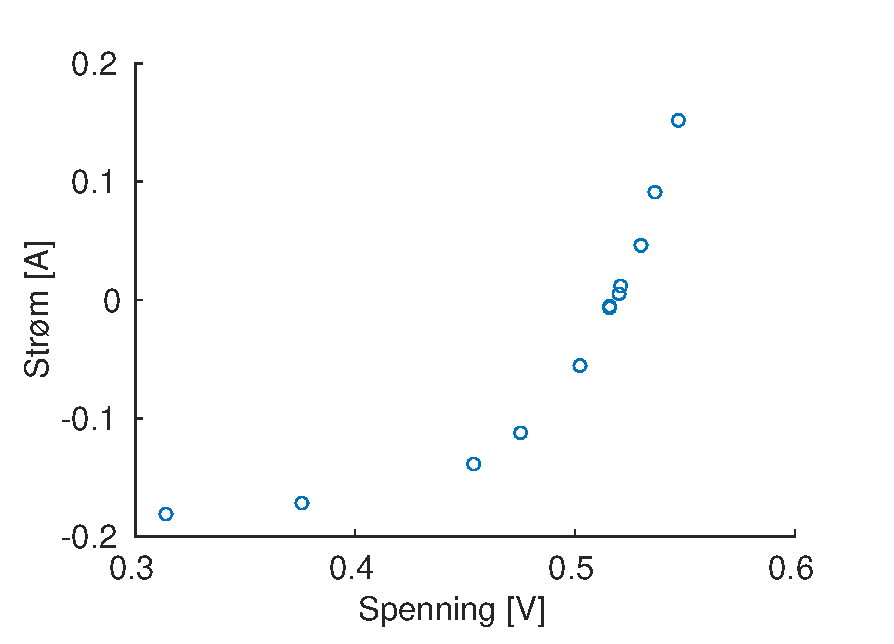
\includegraphics[width = 0.5\textwidth]{matlab/LAB/belystMedSpenning.eps}
	\caption{Strøm-spenning-karakteristikk for belyst solcelle med påtrykt spenning.}
	\label{fig:resMedSpenning}
\end{figure}

\subsubsection{Uten påtrykt spenning}
Figur \ref{fig:resUtenSpenning} viser strøm-spenning-karakteristikk for solcellen både med og uten påtrykt spenning.
\begin{figure}[!ht]
	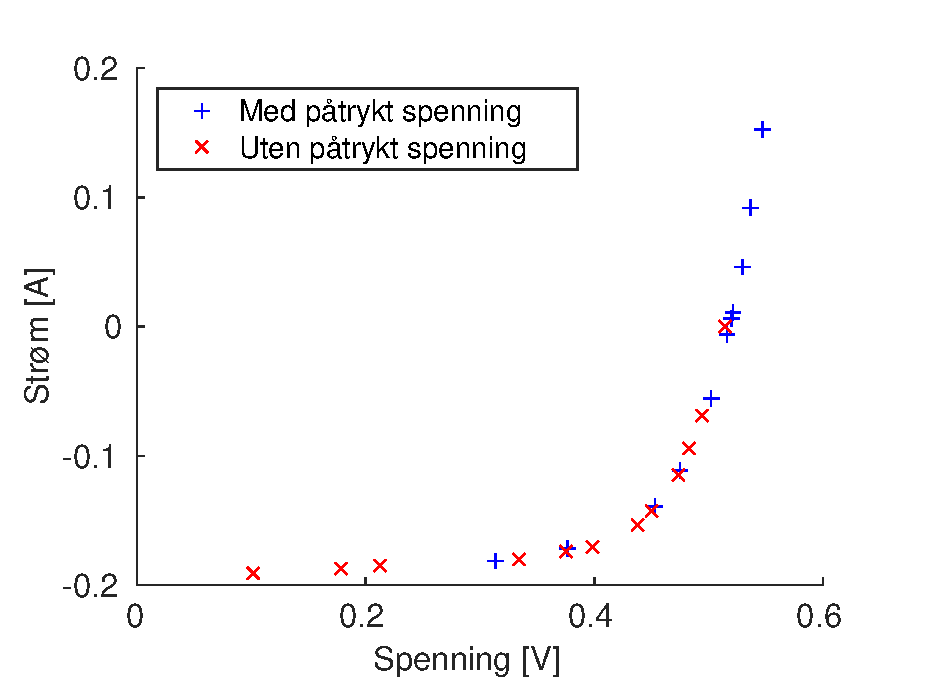
\includegraphics[width = 0.5\textwidth]{matlab/LAB/utenSpenning.eps}
	\caption{Strøm-spenning-karakteristikk for belyst solcelle med og uten påtrykt spenning.}
	\label{fig:resUtenSpenning}
\end{figure}

\subsection{Solcellens optimale belastning}
Strøm-spenning-karakteristikken til den roterte solcellen er plottet i figur \ref{fig:currentVoltageRotation}, sammen med samme karakteristikk for solcellen under full belysning.

\begin{figure}[!ht]
	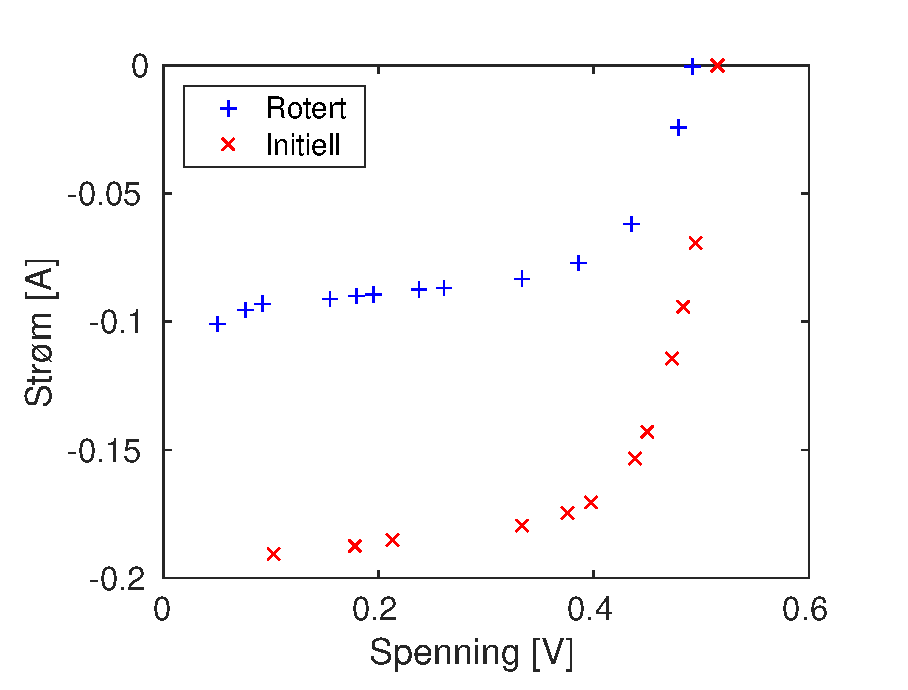
\includegraphics[width = 0.5\textwidth]{matlab/LAB/currentVoltageRotated.eps}
	\caption{Strøm-spenning-karakteristikk for solcellen før og etter rotasjon.}
	\label{fig:currentVoltageRotation}
\end{figure}

Figur \ref{fig:effekt} viser sammenhengen mellom spenning og effekt for solcellen ved full og redusert belysning. Maksimal effekt fant vi ved 7$\Omega$ og 2.2$\Omega$, for henholdsvis redusert og full belysning.
\begin{figure}[!ht]
	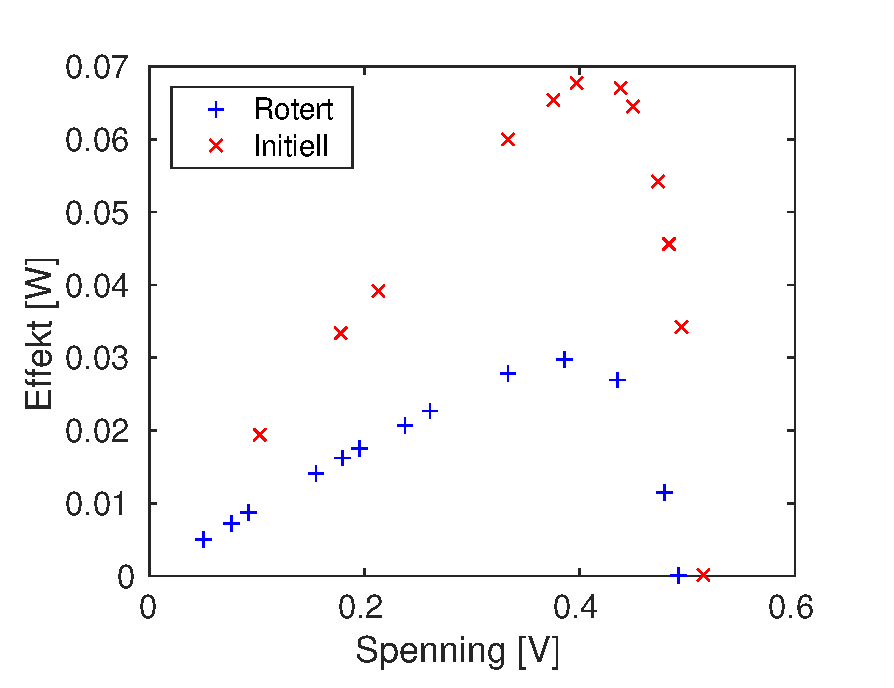
\includegraphics[width = 0.5\textwidth]{matlab/LAB/optimalBelastning.eps}
	\caption{Effekt som funksjon av spenning for solcellen under full og redusert belysning.}
	\label{fig:effekt}
\end{figure}

\subsection{Kombinasjon av solceller}
Resultatene for målinger på parallell- og seriekoblede solceller er presentert i tabell \ref{tab:serieParallell}. Spenningen over lasten er bare målt for en lastmotstand på $0.5\Omega$

\begin{table}[!ht]
	\caption{Resultater for måling av parallellkoblet (p) krets og seriekoblet (s) krets for to belyste solceller og \'en belyst solcelle.}
	\label{tab:serieParallell}
	\begin{tabular}{lccc}
		\toprule
		\toprule
		Kobling & $V_L$[mV]  & $I_\text{sc}$[mA] & $V_\text{oc}$[mV]\\
		\hline
		To belyst$_\text{p}$ & 193.1  & 386.2 & 514.8\\
		To belyst$_\text{s}$ &  96  & 192 & 1028\\
		\'En belyst$_\text{p}$ &  99.7  & 199.4 & 491.7\\
		\'En belyst$_\text{s}$ &  0.21  & 0.42 & 618\\
		\toprule
	\end{tabular}
\end{table}

Vi benytter nå ligning \eqref{eq:forhold} til å bestemme forholdet mellom den maksimale effekten mellom to belyste celler og \'en belyst celle. 

For parallellkobling har vi 
\begin{equation}
	\frac{P_\text{max, to belyst}}{P_\text{max, \'en belyst}} = \frac{514.8\cdot386.2}{491.7\cdot199.4} = 2.03
\end{equation}

For seriekobling har vi 
\begin{equation}
	\frac{P_\text{max, to belyst}}{P_\text{max, \'en belyst}} = \frac{1028\cdot2056}{0.42\cdot618} = 8142
\end{equation}
Vi kan bruke samme ligning til å se på forholdet mellom serie- og parallellkobling der begge cellene er belyst for begge kretsene.
\begin{equation}
	\frac{P_\text{max, parallell}}{P_\text{max, serie}} = \frac{514.8\cdot386.2}{1028\cdot192} = 1.01
\end{equation}
Omtrentlige tall fra figur \ref{fig:resUtenSpenning} gir at vi for \'en  belyst solcelle i en enkel krets har $V_\text{oc}=515$mV og $I_\text{sc}=190$mA. Så hvis vi sammenligner effekten til en enkelt solcelle i forhold til to i parallell får vi
\begin{equation}
	\frac{P_\text{max, parallell}}{P_\text{max, enkelt}} = \frac{514.8\cdot386.2}{515\cdot190} = 2.03
\end{equation}
\subsection{Solcellens effektivitet}
For å finne ut hvor stor effektivitet en solcelle har så må vi først vite arealet til cellen. Figur \ref{fig:solcelleoverflate} viser en skisse av overflaten til solcellen, og hvilke verdier vi målte for lengdene.
\begin{figure}[!ht]
\centering
	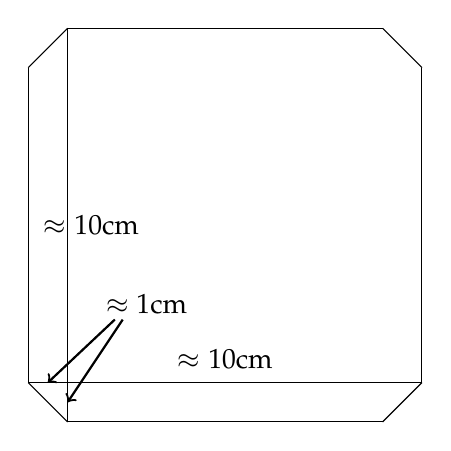
\begin{tikzpicture}
		\draw (0.5,0)--(4.5,0);
		\draw (4.5,0)--(5,0.5);
		\draw (5,0.5)--(5,4.5);
		\draw (5,4.5)--(4.5,5);
		\draw (4.5,5)--(0.5,5);
		\draw (0.5,5)--(0,4.5);
		\draw (0,4.5)--(0,0.5);
		\draw (0,0.5)--(0.5,0);
		%Målte lengder
		\draw (0,0.5)--(5,0.5);
		\draw (0.5,5)--(0.5,0);
		\node (l) at (2.5, 0.8) {$\approx10$cm};
		\node (h) at (0.8, 2.5) {$\approx10$cm};
		\node (t) at (1.5,1.5) {$\approx1$cm};
		\draw [thick, ->] (1.1,1.3) -- (0.25, 0.5);
		\draw [thick, ->] (1.2,1.3) -- (0.5, 0.25);
	\end{tikzpicture}
	\caption{Solcellens overflate med estimerte mål}
	\label{fig:solcelleoverflate}
\end{figure}
Vi finner et areal for solcellen på
\begin{align}
	A &\approx (10\text{cm}^2)-4\cdot\frac{(1\text{cm})^2}{2}\\
	&= 98\text{cm}^2 = \underline{98\cdot 10^{-4}\text{m}^2}
\end{align}

Videre fant vi den maksimale effekten fra data vi allerede hadde funnet i forsøket med enkelt belyst solcelle, uten påtrykt spenning. Denne effekten fant vi til å være 0.068W. Solarimeteret viste 0.363mV. Dermed blir solcellen bestrålt med en effekt på
\begin{equation}
	P_\text{inn} = \frac{0.363\text{mV}\cdot98\cdot10^{-4}\text{m}^2}{4.84\cdot10^{-3}\text{mV/Wm}^{-2}} = 0.735W
\end{equation}

Virkningsgraden til solcellen blir dermed
\begin{equation}
	\eta = \frac{P_\text{max}}{P_\text{inn}} = \frac{0.068W}{0.735W} = 9.25\text{\%}
\end{equation}
Videre betrakter vi samme oppsett, men filtrer lyset fra kilden med to forskjellige fargefilter.
\subsubsection{Blått fargefilter}
Solarimeteret viste en spenning på på 0.012\text{mV}. Dette gir en innlyst effekt på 0.0243W, regnet på samme måte som over. Vi fant spenningskurven vist i figur \ref{fig:effektBlue} og avgjorde fra denne og dataene at den maksimale effekten var på 0.0016W. Vi får dermed en virkningsgrad på 
\begin{equation}
	\eta = \frac{0.0016\text{W}}{0.0243\text{W}} = 6.6\text{\%}
\end{equation}
\begin{figure}[!ht]
	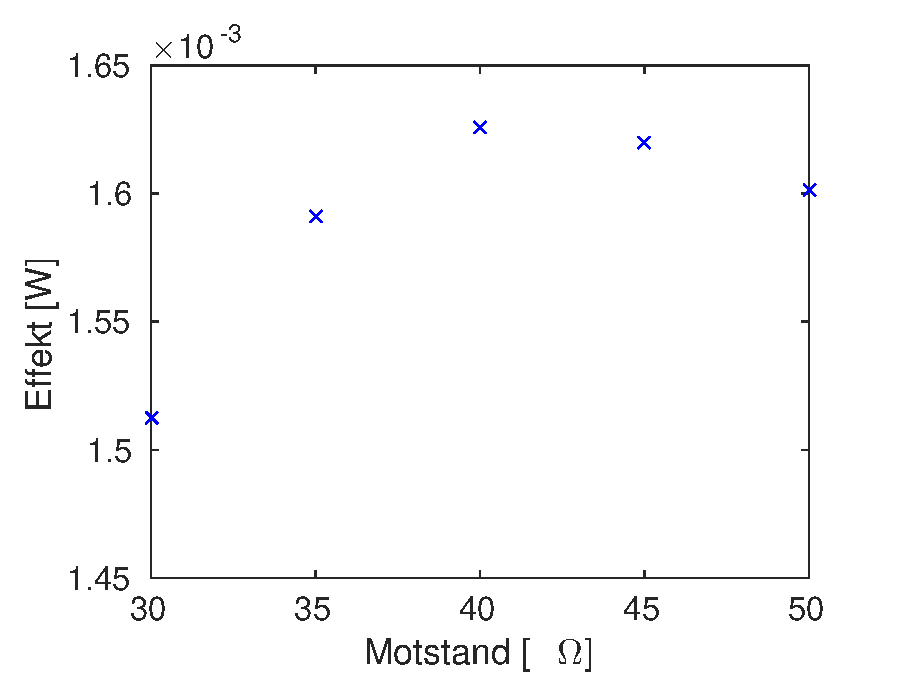
\includegraphics[width = 0.5\textwidth]{matlab/LAB/effektBlue.eps}
	\caption{Effekt som funksjon av lastmotstand for blått fargefilter.}
	\label{fig:effektBlue}
\end{figure}
\subsubsection{Rødt fargefilter}
Solarimeteret viste en spenning på på 0.047\text{mV}. Dette gir en innlyst effekt på 0.0952W, regnet på samme måte som over.
\begin{figure}[!ht]
	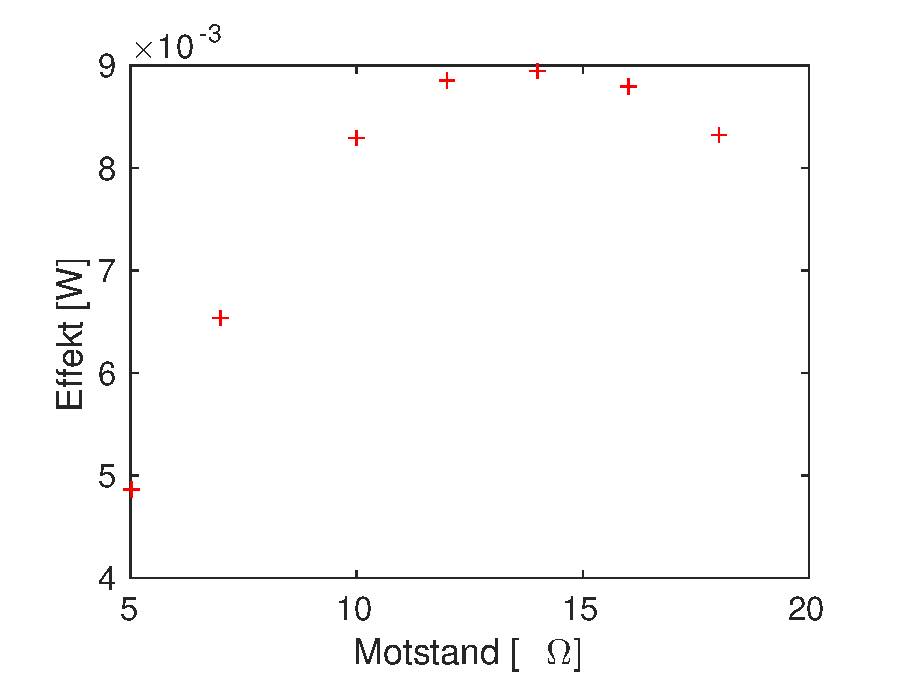
\includegraphics[width = 0.5\textwidth]{matlab/LAB/effektRed.eps}
	\caption{Effekt som funksjon av lastmotstand for rødt fargefilter.}
	\label{fig:effektRed}
\end{figure}
Ved å betrakte figur \ref{fig:effektRed} og dataene punktene plottet består av finner vi en maksimal effekt på 0.009W. Dermed får vi en virkningsgrad på 
\begin{equation}
	\eta = \frac{0.009\text{W}}{0.0952W} = 9.5\text{\%}
\end{equation}
\section{Diskusjon}
\subsection{Strøm-spenning-karakteristikken}
Vi kunne nok ha valgt enda bedre punkter for målingene våre med påtrykt spenning. Det viktige området viser seg å ligge mellom 0.4 og 0.5V. Dette området ble dekt bedre for målingene uten påtrykt spenning. 

Av figur \ref{fig:resUtenSpenning}, som viser plot for solcellen både med og uten påtrykt spenning, ser vi at karakteristikkene sammenfaller. Vi finner selvfølgelig ikke de positive strømmene for solcellen uten påtrykt spenning, og heller ikke negative spenninger, men i fjerde kvadrant er karakteristikkene mer eller mindre like. Dette er naturlig ettersom oppførselen til solcellen i forhold til hvor mye strøm som går gjennom den i hovedsak avhenger av spenningen over cellen. Vi oppnår disse spenningene ved forskjellig lastmotstand for kretsen med og uten påtrykt spenning, men den resulterende karakteristikken i det gjeldende området blir den samme.

\subsection{Solcellens optimale belastning}
Vi ser fra resultatene at den optimale lastmotstanden til solcellen forandrer seg med belysningen, med tanke på å produsere mest mulig effekt. Det er dermed ikke optimalt å belaste solcellen med den samme resistansen hele tiden. En grei mulighet for å lage en reguleringskrets ville vært å la solcellen levere variabel strøm under konstant spenning. Fra figur \ref{fig:effekt} ser vi at maksimal effekt levert fra solcellen er ved ca. samme spenning for de to forskjellige belysningene. Figur \ref{fig:currentVoltageRotation} viser oss at redusert belysning gir oss drastiske forandringer i strømmen, mens spenningen forblir omtrent den samme. Fra samme figur ser vi også at det er problematisk å sette en konstant strøm for å oppnå maksimalt areal innenfor begge karakteristikkene, men at det går helt greit med konstant spenning.

\subsection{Kombinasjon av solceller}
Fra resultatene våre finner vi at både parallell- og seriekobling vil gi en proporsjonal øking av effekt. For parallellkobling forsvinner den effekten som en solcelle gir hvis den tildekkes slik at den ikke mottar lys. Hvis solcellene derimot er koblet i serie så vil bortimot all effekten forsvinne dersom så lite som \'en av cellene dekkes til. Dette er fordi kretsen nærmest blir kortsluttet når solcellen ikke er belyst, slik at det ikke går noen strøm i kretsen.

\subsection{Solcellens effektivitet} 

%\printbibliography
\clearpage
\onecolumn
\appendix


%\section{Matlab-script}

\end{document}
